\chapter{Fire science basics}

In a given year, about 3\% of Earth's terrestrial surface burns \citep{archibald2018}.
All this fire affects air quality, alters vegetation, and drives processes such as climate and nutrient cycles \citep{sullivan2012}. 
A basic understanding of how fire burns is important for anyone involved in wildland fire science and management. 
The first part of this chapter introduces the processes of combustion, heat transfer, and fire spread.
The second part introduces some basics of how scientists measure and describe wildland fire. 

\section{Fire in space and time}

When conducting any type of fire science, one must be aware of multiple spatial and temporal scales at once. 
It is important to consider individual fires within the broader context of biogeography and climate, as well as consider the location of individual sample points within the landscape context of the individual fire. 
Thoughtful placement and timing\textemdash spatial and temporal considerations, respectively\textemdash of samples helps data from one fire fit into knowledge of many fires. 

\begin{figure}
	\begin{center}
		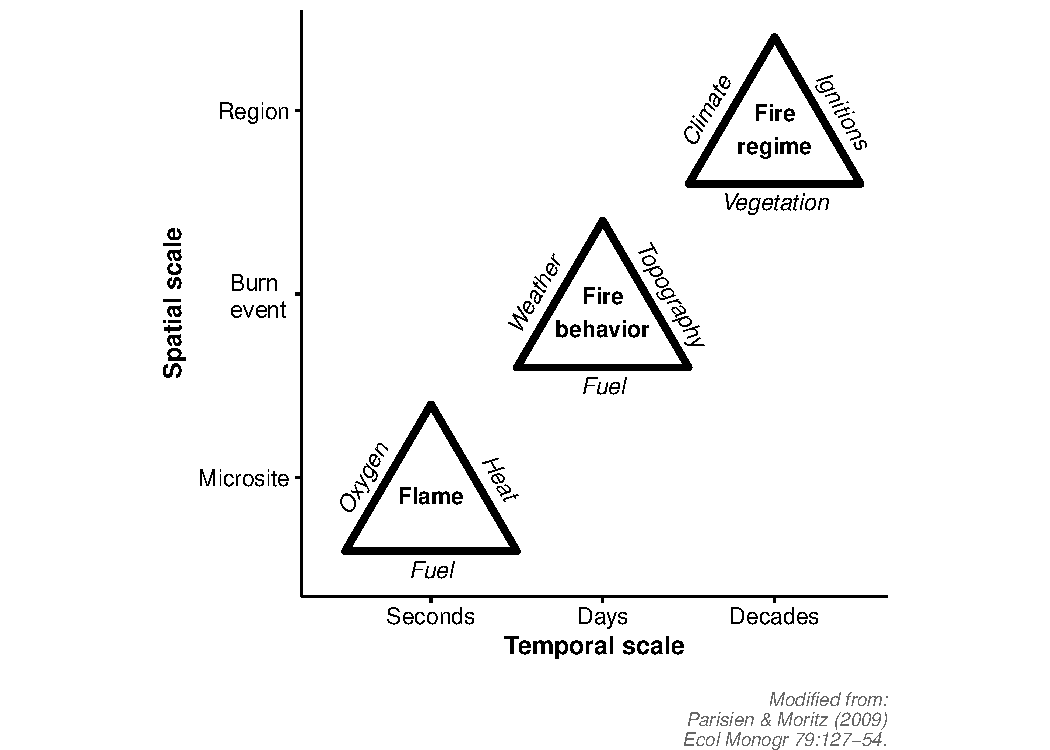
\includegraphics[width=1\columnwidth, 
		trim={2.75cm 1.5cm 2cm 0.5cm}, clip=true]
		{science/FlameTriangles-1}
		%(Fig.~\ref{fig:FireTriangles})
	\end{center}
	\caption{Three scales of wildland fire. Modified from \citet{parisien2009}.
		\label{fig:FireTriangles}}
\end{figure}

The story of fire in a landscape unfolds at three spatio-temporal scales (Fig.~\ref{fig:FireTriangles}). 
Each scale is relevant to the fire scientist. 
The finest and fastest scale is that of individual flames and the movement of the \emph{flaming front}, the series of ignitions that propagate fire through the fuelbed, and across the landscape. 

In prescribed fire, most personnel and planning focus on the middle triangle\textemdash the factors that affect how a fire behaves within the defined burn unit within the operational time period (often less than 1 day). 
How wind, topography, and fuel affect fire behavior is discussed in detail in the fire behavior chapter. 

Good fire management bases broad objectives within a model \emph{fire regime}, which is discussed in more detail later in this chapter. 
Within a given climate and vegetation type (e.g., grassland, savanna, or forest), managers often have fairly specific goals they desire to achieve, and various elements of prescribed fire can be manipulated to serve those goals. 
For example, both the season in which a burn occurs and the ignition pattern used to set it can affect the intensity of the prescribed fire. 
But burns in different seasons can target plants at different stages in their life cycles, as well, so clearly these two elements of the fire regime have important interactions in determining the ultimate effects of a single fire, and especially over time, if fires are repeated. 
Collecting quality data from the fire environment before and during a fire can provide a lot of information to fire managers about what their burns are doing, and how to better plan future operations to increase their chances to achieve their goals. 

\section{What is fire?}

All fire results from the combination of the three fundamental components of the Flame Triangle: Fuel, heat, and oxygen (Fig.~\ref{fig:FireTriangles}).
In the wildland fire environment, fuel consists of plant material. 
The ambient air provides oxygen.
Wind can increase oxygen input, while physical barriers can block air flow. 
Heat must come from an ignition such as lightning or an incendiary device, or from an already-burning fire nearby.

\subsection{Combustion} 

Combustion is a chemical reaction in which the rapid oxidation of plant material produces energy as heat:  

\begin{equation}\label{eq:combustion}
	(C_{6}H_{10}O_{5})_{n} + O_{2} + \text{energy}_{\substack{kindling\\temperature}} \rightarrow   CO_{2} + H_{2}O + \text{energy}_{heat}
\end{equation} 

The left-hand side of Eq.~\ref{eq:combustion} is simply the three components of the flame triangle in Fig.~\ref{fig:FireTriangles}: 

\begin{itemize}
	\item $C_{6}H_{10}O_{5}$ is the chemical formula for cellulose, which represents plant material as fuel. 
	\item Oxygen $O_{2}$ comes from the air. 
	\item \emph{Kindling temperature} is what fuel must be heated to before it ignites and combustion proceeds as a self-sustaining reaction (\~500\degC).
\end{itemize}

Note that in this format, combustion is the reverse of \emph{photosynthesis}, the processes that assembled the plant material in the first place:

\begin{equation}\label{eq:photosynthesis}
	CO_{2} + H_{2}O + \text{energy}_{solar} \rightarrow (C_{6}H_{10}O_{5})_{n} + O_{2}
\end{equation}

Thus, burning plant biomass\textemdash i.e., \emph{combustion}, Eq.~\ref{eq:combustion}\textemdash is just a natural decomposition process that breaks down vegetation. 

Combustion can be divided into distinct phases:\footnote{It is important to keep in mind that \textit{combustion in the wildland environment is not linear}. 
	Because vegetation has all sorts of sizes, arrangements, and chemical and moisture contents, wildland fuel particles heat unevenly and release gases and energy at different rates \citep{sullivan2012, finney2013}.
	In fact, fire ecologists have used an overly-simple model of combustion for decades \citep{sullivan2017}, which often focuses on changes in temperature.
	But combustion is better understood as the exchange of energy between the environment and plant matter at the surface of fuel particles, known as the \emph{reaction zone}. 
	These review papers really get into the complexities of wildland fuel combustion: \citep{sullivan2012, sullivan2017, sullivan2017a}.  
} 

\begin{enumerate} 
	\item \textbf{Preheating\textemdash}Fuel particles begin to absorb heat. Dehydration begins at 100\degC\textemdash moisture is driven out of fuel particles. This is an \emph{endothermic} part of the process, meaning it depends on heat from an external source. Often the energy source is an approaching flame front, so the heating rate increases as the flame front approaches. Flame contact leads to rapid heating. 
	\item \textbf{Pyrolysis\textemdash}The thermal degradation of matter. Around 200\degC, chemical bonds in the fuel start to break down. The fuel particle begins to lose mass as previously solid components like cellulose volatilize. Around 500\degC, any remaining material essentially turns into charcoal. 
	\item \textbf{Ignition\textemdash}The endothermic reaction that required heat input transitions to an \emph{exothermic} reaction that releases heat. More than just reaching a threshold temperature (e.g., \emph{kindling temperature}, as in Eq.~\ref{eq:combustion}), this phase means the reaction is releasing energy faster than the surrounding environment can absorb it.
	\item \textbf{Flaming combustion\textemdash}The reaction zone\textemdash the surface of the fuel particle between 200\textendash 500\degC\textemdash is engulfed in flame as the heated gases released by pyrolysis mix with oxygen in the air and ignite.
	\item \textbf{Glowing combustion\textemdash}Remainder of solid fuel particles continue to break down, even after all the gases have been released and burnt off as flames. Also known as \emph{smoldering}. 
	\item \textbf{Extinction\textemdash}Combustion finally ceases, but not necessarily because all of the fuel is gone. Once the reaction no longer produces energy faster than it can be absorbed by any moisture or inorganic materials nearby, the reaction will slow and the fuel particle will cool enough to stop combustion if no more energy is added. 
\end{enumerate}

\subsection{Heat transfer}

	\index{Heat transfer|textbf}
No matter how hot a fuel particle burns, wildland fire cannot spread unless heat energy transfers to another fuel particle. 
The transfer of heat energy from combusting fuel to adjacent particles is called \emph{propagation}. 
Heat transfer in the wildland fire environment follows three standard physical processes (Fig.~\ref{fig:HeatTransfer}): 
	\index{Propagation|textbf}

\begin{figure}
	\caption{
		The three basic mechanisms of heat transfer. Convection is often the most important mechanism in wildland fire: buoyant hot air moves uphill or is pushed ahead of the fire by wind to preheat fuels prior to contact with flames. 		  
		\label{fig:HeatTransfer} }
	\begin{center}
		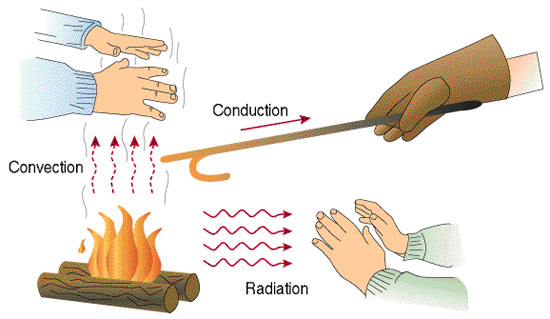
\includegraphics[width=1\textwidth, trim={0cm 0cm 0cm 0cm}, clip=true]{science/HeatTransfer}
			\PhotoCredit{Kmecfiunit CC BY-SA 4.0}
			\PhotoIndex{CC BY-SA 4.0}
		{fig:HeatTransfer}
		{Kmecfiunit}
		{https://upload.wikimedia.org/wikipedia/commons/e/e6/Heat-transmittance-means1.jpg}
		%(Fig.~\ref{fig:HeatTransfer})
	\end{center}
\end{figure}

\begin{itemize}
	\item \textbf{Conduction\textemdash}The transfer of heat through direct contact, from molecule to molecule within an object. Since plant matter generally conducts heat poorly, especially when dry, conduction in the wildland fire environment is primarily limited to carrying heat through soil and large-diameter fuels like logs. 
	\item \textbf{Convection\textemdash}The transfer of heat through air flow is important in determining the direction of fire spread.\footnote{As further evidence of the complexity of the wildland fire environment, convection can also \emph{cool} fuel particles that are being heated by other processes, and the relative influence of heat loss vs. heat gain increases with the surface area:volume ratio of the fuel particle \citep{finney2013}.} \emph{Free convection} is the buoyant rise of heated air; \emph{forced convection} is hot air moved by wind.
	\item \textbf{Radiation\textemdash}The transfer of energy via electromagnetic waves.While radiation can occur over relatively long distances, it requires unhindered line-of-sight movement and is thus limited to much shorter ranges in dense fuels. 
\end{itemize}

\begin{figure}
	\caption{
		Flame pulsation 		  
		\label{fig:FlamePulsation} }
	\begin{center}
		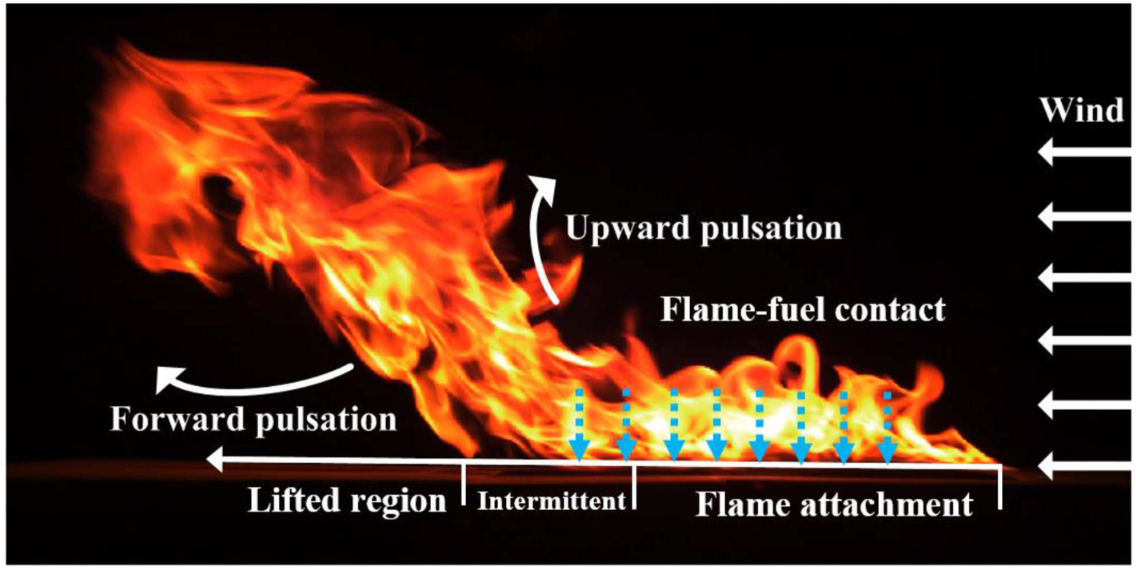
\includegraphics[width=1\textwidth, 
		trim={0cm 0cm 0cm 0cm}, clip=true]
		{science/FlamePulsation}
		\PhotoCredit{\citet{tang2019}, CC BY 4.0}
		\PhotoIndex{CC BY 4.0}
		{fig:FlamePulsation}
		{\citet{tang2019}}
		{https://www.frontiersin.org/articles/10.3389/fmech.2019.00034/full}
		%(Fig.~\ref{fig:FlamePulsation})
	\end{center}
\end{figure}

Two other heat transfer mechanisms are also important in the wildland fire environment:

\begin{itemize}
	\item \textbf{Direct flame contact} is critical to propagation as it can ignite particles ahead of the flame front (Fig.~\ref{fig:FlamePulsation}). Flames can be pushed forward by wind, or even by a fire's own fluid dynamics. 
	Brief, fine-scale turbulent pulsations created by fresh air flowing into the reaction zone as buoyant hot air lifts away can create horizontal vortices that push flames down, into contact with pre-heated fuel particles. The flame contact rapidly bringing them up to ignition temperature.\footnote{\citet{finney2015, tang2017, morandini2018}} 
	\item \textbf{Solid fuel transport} is the physical movement and deposition of burning fuel particles: 
	\begin{itemize}
		\item Large burning particles can break apart as pyrolysis degrades them; these burning chunks can fall or roll and cause ignition downhill.
		\item \emph{Firebrands}, or burning embers, can get carried by wind and fall far from the original fire. When firebrands land in a receptive fuelbed that is dry enough to ignite, they start \emph{spot fires}.
	\end{itemize}
\end{itemize}

\section{Wildland fuels} 

	\index{Fuel!Fuel characteristics|textbf}
Wildland fuels are comprised of plant material. 
There are many species of plants, and they take many forms. 
Thus many properties describe wildland fuels: vegetation type (e.g., grasses, brush, coniferous or deciduous trees, logging slash, etc.); arrangement and structure (e.g., horizontal or vertical, continuous or discontinuous); particle size, along with surface area to volume ratio; particle density (loft, or packing ratio); whether the vegetation is alive or dead, standing or fallen, and whether it was derived from leaves or stems. 
But since fire spread depends on the transfer of heat energy through the environment, the diversity of plants can be functionally reduced to just a few categories of wildland fuel based on their thermal properties. 

\subsection{Fuel size classes} 

\index{Fuel!Fuel characteristics!Size classes|textbf}

\begin{marginfigure}
	\begin{center}
		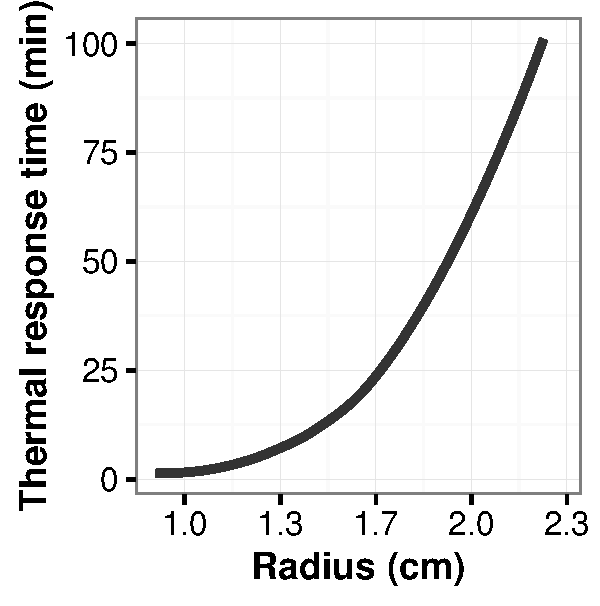
\includegraphics[width=1\textwidth, 
		trim={0cm 0cm 0cm 0},clip=true]
		{science/fosberg1973-1}
		\DataCredit{\citet{fosberg1973}}
		\caption{The non-linear relationship between fuel particle size and heat transfer rate.
			Small increases in fuel particle radius leads to disproportionately large increases in thermal response time\textemdash the speed at which the material changes temperature. 
			Thus, a fuel particle with radius 1 cm has a response time of 1.4 min, while  the response time jumps to 56 min for a particle of 2 cm radius. } \label{fig:Fosberg1973}
	\end{center}
\end{marginfigure} 

The primary categorization is \emph{size class}, which is given by a fuel particle's diameter.
Different diameters produce different surface area:volume ratios, which affects heat transfer rates: both how quickly the particle gains heat during pre-heating (Fig.~\ref{fig:Fosberg1973}), and the rate at which heat is lost while smoldering prior to extinction. 
Fuel size classes are referred to by their \emph{lag times}, which refers to how quickly fuel particles gain and lose heat and moisture.
The size classes of fuel are 1-hour, 10-hour, and 100-hour, which correspond to diameters of $<$ 0.6 cm,  0.6\textendash 2.5 cm, and 2.5\textendash 7.6 cm, respectively \citep{fosberg1971}.\footnote{The metric delineations might seem odd, but the original categories were in inches: $<$ 0.25, 0.25\textendash 1, 1\textendash 3. Some recognize a 1,000-hr class for very large fuels.}

It is often sufficient to differentiate fine fuel (1-hr) from coarse fuel (10-hr and above). 
Physically, fine fuels are ``thermally thin'', with low surface area:volume ratios that take on heat quickly and evenly, and have often fully combusted by the time the flame front passes. 
In the field, the fine/coarse distinction might apply to grasses vs. larger shrubs, trees, and downed woody debris.\footnote{
In prescribed fire, fine and coarse fuels are often managed separately\textemdash undesired woody plants might be targeted for heating, while desired species are to be protected, and keeping a pile of woody debris from igniting in the first place is the best way to ensure it doesn't kick up embers hours after everyone has gone home.}

\subsection{Fuel moisture}
\index{Fuel!Fuel moisture|textbf}

Fuel moisture is an important property, and wildland fuel moisture dynamics follow the size classes described above. 
\index{Fuel!Fuel types!Dead fuels}
\index{Fuel!Fuel types!Live fuels}
But first it is important to distinguish between living versus dead vegetation. 
There are two reasons fuels ought to be considered a class by themselves \citep{finney2013}:\sidenote{
	Fire scientists have struggled to account for live vegetation.
	In the parlance of wildland fire science, live fuels are often \emph{not available to burn} because they are insufficiently \emph{cured}, i.e. they haven't been dried out through exposure to warm air or radiation. 
	Because many management fires occur outside of dry, dormant seasons or in fuelbeds dominated by invasive species, prescribed fire managers (and scientists) must think beyond dead fuels alone. } 
\begin{itemize}
	\item Moisture in living plant tissue is under the biological control of the organism (ecophysiology), whereas dead fuel moisture is a passive interaction between plant tissue and the environment.
	\item Live tissue moisture often exceeds levels that will support combustion\textemdash in terms of heat flux, this moisture absorbs energy, making living plant tissue more of a sink than a source of combustion energy.
	And live tissues retain this moisture until their cells fail, slowing dehydration.  
\end{itemize}

\index{Lag times|see {Fuel characteristics, size classes}} 
\index{Fuel!Fuel characteristics!Size classes}
Within dead fuels, the concept of lag times applies to fuel moisture gain and loss as well as heating and cooling: dead fuel moisture depends on the moisture content of the air around it. 
All dead fuels passively gain and lose moisture by exposure to the atmosphere, and fine dead fuel moisture changes faster than coarse fuels. 

Several environmental variables affect fuel moisture transfer rates.
\index{Weather!Relative humidity}
\index{Weather!Precipitation}
Sources of moisture include the atmosphere itself\textemdash humidity and precipitation\textemdash and contact with other sources capable of holding and releasing moisture, such as soil and forest duff.
\index{Fuel!Fuel characteristics!Equilibrium moisture content}
\index{Equilibrium moisture content|see {Fuel characteristics}} 
When these sources are steady, fuel particles eventually reach an \emph{equilibrium moisture content} with the surrounding air\textemdash gains and losses of moisture via diffusion with the air are net neutral. 
Fine fuels reach equilibrium moisture content within a matter of hours, while coarse fuel can take days or weeks to become available for combustion if they got soaked through.
Drying increases with exposure to both wind and solar radiation \citep{byram1943}.

\subsection{The fuelbed and fire types}

\index{Fuel!Fuelbed|textbf} 
Wildland fuels occupy a three-dimensional space called the \emph{fuelbed} through which flame fronts spread from particle to particle. 
As such, the structure of plant biomass in this three-dimensional space has a major effect on fire. 
Within the landscape, the type of vegetation\textemdash grassland, brush, or forest\textemdash determines the type of fuel available to burn. 
Within the combustion reaction zone, the arrangement and density of fuel particles regulate the flame triangle\textemdash fuel availability, oxygen flow, and how quickly heat transfers to new fuel particles.  

\index{Fire types|textbf}
\index{Fire types!Ground fire}
\index{Fire types!Surface fire}
Three broad fire types are defined by the fuel layer through which fire spreads (Fig. \ref{fig:FireTypes}): \emph{ground fires} burn through organic material below the soil surface, such as peat and heavy forest duff; \emph{surface fires} burn through herbaceous and brushy aboveground plant biomass rooted in, or laying on, the soil surface; and \emph{canopy fires} burn through the foliage of standing trees; \emph{torching} is when the canopy of a single tree burns, while fire propagating from one canopy to another \emph{running crown fire}. 
Although fire rarely starts in the canopy, canopy fuels can be ignited by extremely high surface flames or via \emph{ladder fuels}\textemdash hanging branches, vines, or shrubs and trees of younger age classes that carry fire into the canopy after first being ignited on the surface. \index{Fuel!Fuel types!Ladder fuels} 
These canopy dynamics are a vivid illustration of the importance of \emph{horizontal continuity}\textemdash how far apart the trees are\textemdash and \emph{vertical continuity} between surface and canopy fuels, but these dynamics are at play in determining surface fire spread and behavior, as well.  

\begin{figure*}
	\begin{center}
		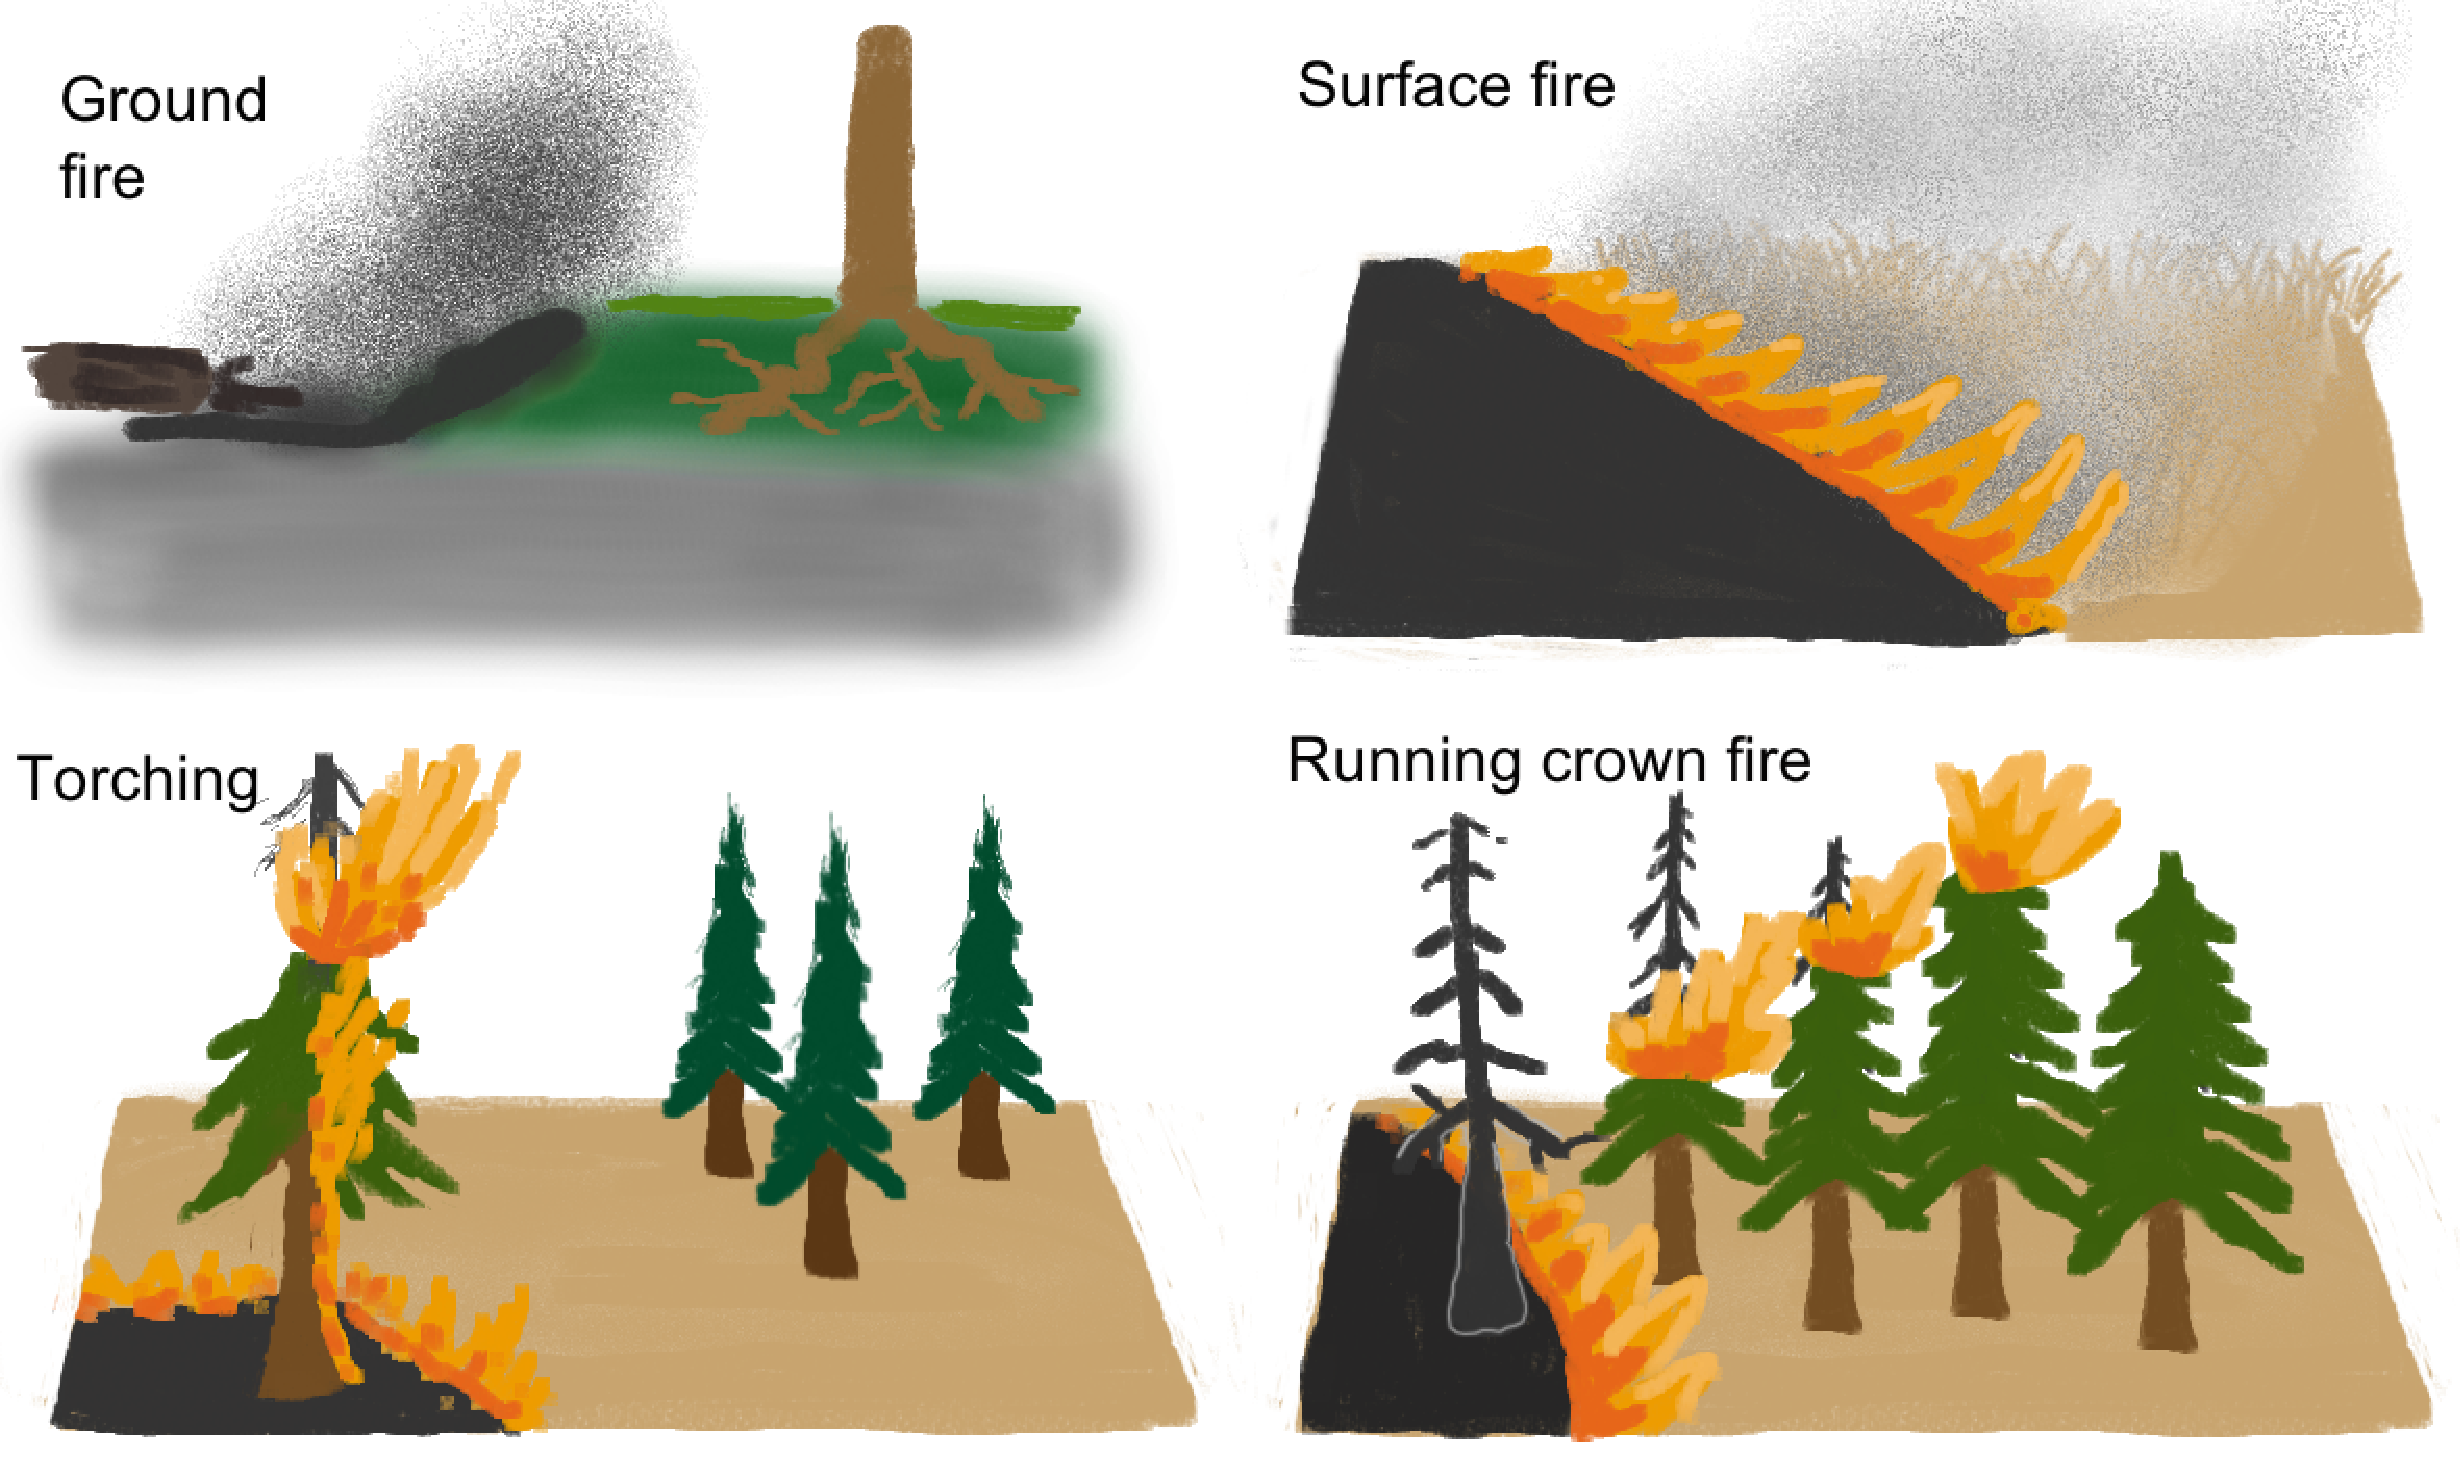
\includegraphics[width=1\textwidth]
		{science/FireTypes}
		%(Fig.~\ref{fig:FireTypes})
	\end{center}
	\caption{Four types of wildland fires. 
		\emph{Ground fires} burn underground through organic material like peat, while \emph{surface fires} move aboveground through fuels on the soil surface. 
		Fire can transition to tree canopies, as well. 
		\emph{Torching} occurs when the canopy of a single tree burns, while \emph{running crown fires} involve canopies of multiple trees.
		\label{fig:FireTypes}}
\end{figure*} 

\section{Fire behavior}

\index{Fire behavior|textbf}
\emph{Fire behavior} describes energy release by the combustion of vegetation, and is controlled by the three factors in the Fire Behavior Triangle  (Fig.~\ref{fig:FireBehaviorTriangle}).  
With knowledge and experience, wildland fire professionals can learn to anticipate how environmental factors influence fire behavior in a particular fuelbed.

Direct observations include how fast a fire moves, how long fuels burn, and the length of flames. 
Indirect observations include how much unburned fuel is left behind, or how high up trees are scorched by flames.

Two standard descriptors of fire behavior are rate of spread and intensity.
\emph{Rate of spread} is simply how fast the flame front moves through the fuelbed.
\emph{Intensity}\textemdash which is not directly observable \textemdash refers to energy release; specifically, \emph{fireline intensity} is the amount of heat released per length of flame front within a period of time \citep{rothermel1983}.
\index{Fire behaviour!Flame length}
\emph{Flame length} is directly related to the rate of energy release and thus serves as an observable proxy of intensity \citep{rothermel1983}.
Both fireline intensity and flame length increase with fuel load and decrease as fuel moisture increases \citep{kreye2013}.

\begin{marginfigure}
	\begin{center}
		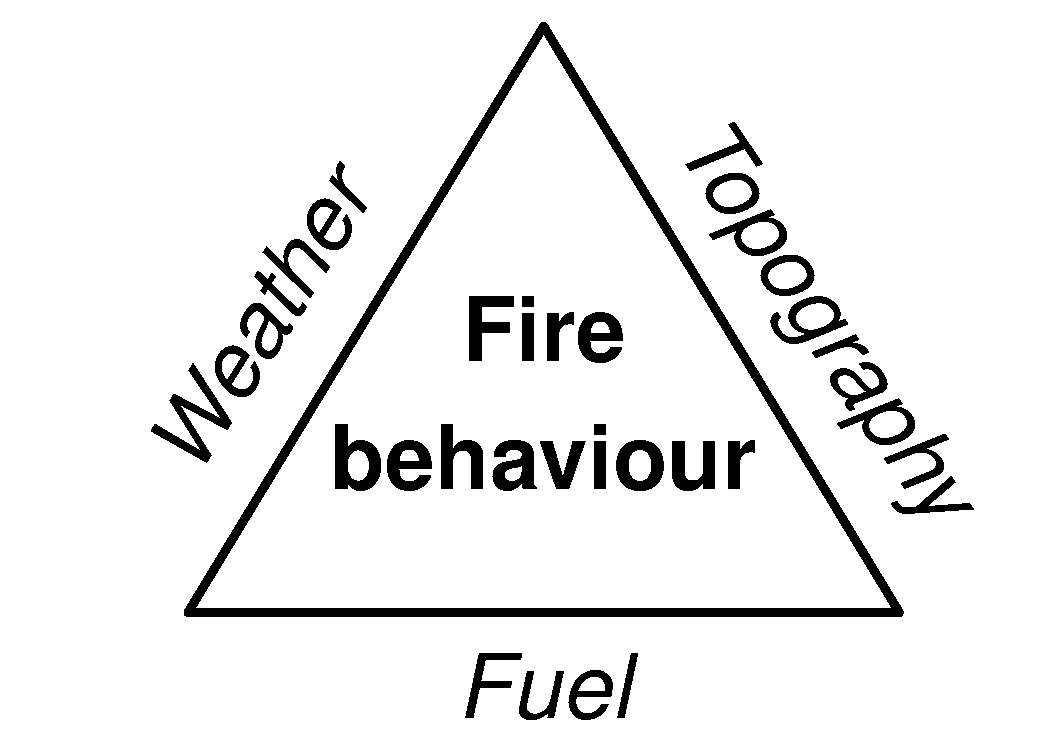
\includegraphics[width=2.2in, 
		trim={1.5cm 0cm 1cm 0.5cm}, clip=true]
		{science/behavior/FireBehaviourTriangle-1}
		\caption{Topography, weather, and the fuelbed are the three major drivers of wildland fire behavior.
			\index{Fire triangles!Fire behavior|textit} \label{fig:FireBehaviorTriangle} } 
		% (Fig.~\ref{fig:FireBehaviorTriangle})
	\end{center}
\end{marginfigure}

When fuels are constant, variability in fire behavior is driven primarily by wind and the flatness or steepness of the terrain, or \emph{slope}. 
Wind and slope are important because they affect heat transfer and facilitate pre-heating, which is the critical mechanism for flame propagation \citep{sancheztarifa1967}. 
Wind pushes heat ahead of the flame front and hot air rises upslope, both of which increase convective heat transfer \citep{sharples2008}.
\index{Heat transfer!Convection} 
\index{Heat transfer!Flames}
Both also reduce the angle between the flame and surface fuels, increasing the probability of heat transfer via flame contact.
The effect is for fires to move faster with the wind, or up a slope, and more slowly against the wind, or down a slope, than in the absence of either.

\section{Wildland fire anatomy} 

	\index{Fuel!Fuelbed}
Because the effects of slope and wind on heat transfer are predictable, one can also predict the shape and direction of wildland fire spread through a given fuelbed.
Fire behavior also varies predictably at different points along the fire perimeter relative to wind direction and slope. 

Assume a single-point ignition in a flat grass fuelbed. 
Without wind, the flame front would slowly spread at a constant rate in all directions. 
Heat transfer is limited to particles very near the reaction zone. 
A fire under a no-wind scenario appears as a slowly-expanding circle. 
But if a wind were to rise, heat transfer rates will vary between the upwind and downwind directions and the shape of the fire becomes elliptical as different parts of the fire spread at different rates (Fig.~\ref{fig:EllipseCartoon}). 

\begin{figure}
	\caption{The anatomy of a surface fire. 
		Here the wind moves from left to right, giving the fire an elliptical shape as the \emph{heading fire} moves fastest with the wind, and has the longest flames. 
		Conversely, the \emph{backing fire} moves the slowest, creeping into the wind. 
		On each side, \emph{flanking fires} spread perpendicular to the wind at a rate between the backing and heading fires; they are aerated by the wind but are neither moving fully against it nor with it. 
		The burned area in the centre of the fire is often called ``the black'' and is an important safety zone for fire personnel due to the lack of remaining fuel. 
		The spot fire was ignited by a \emph{firebrand}, or ember, carried ahead of the main fire by the wind. 
		\label{fig:EllipseCartoon}  }
	\begin{center}
		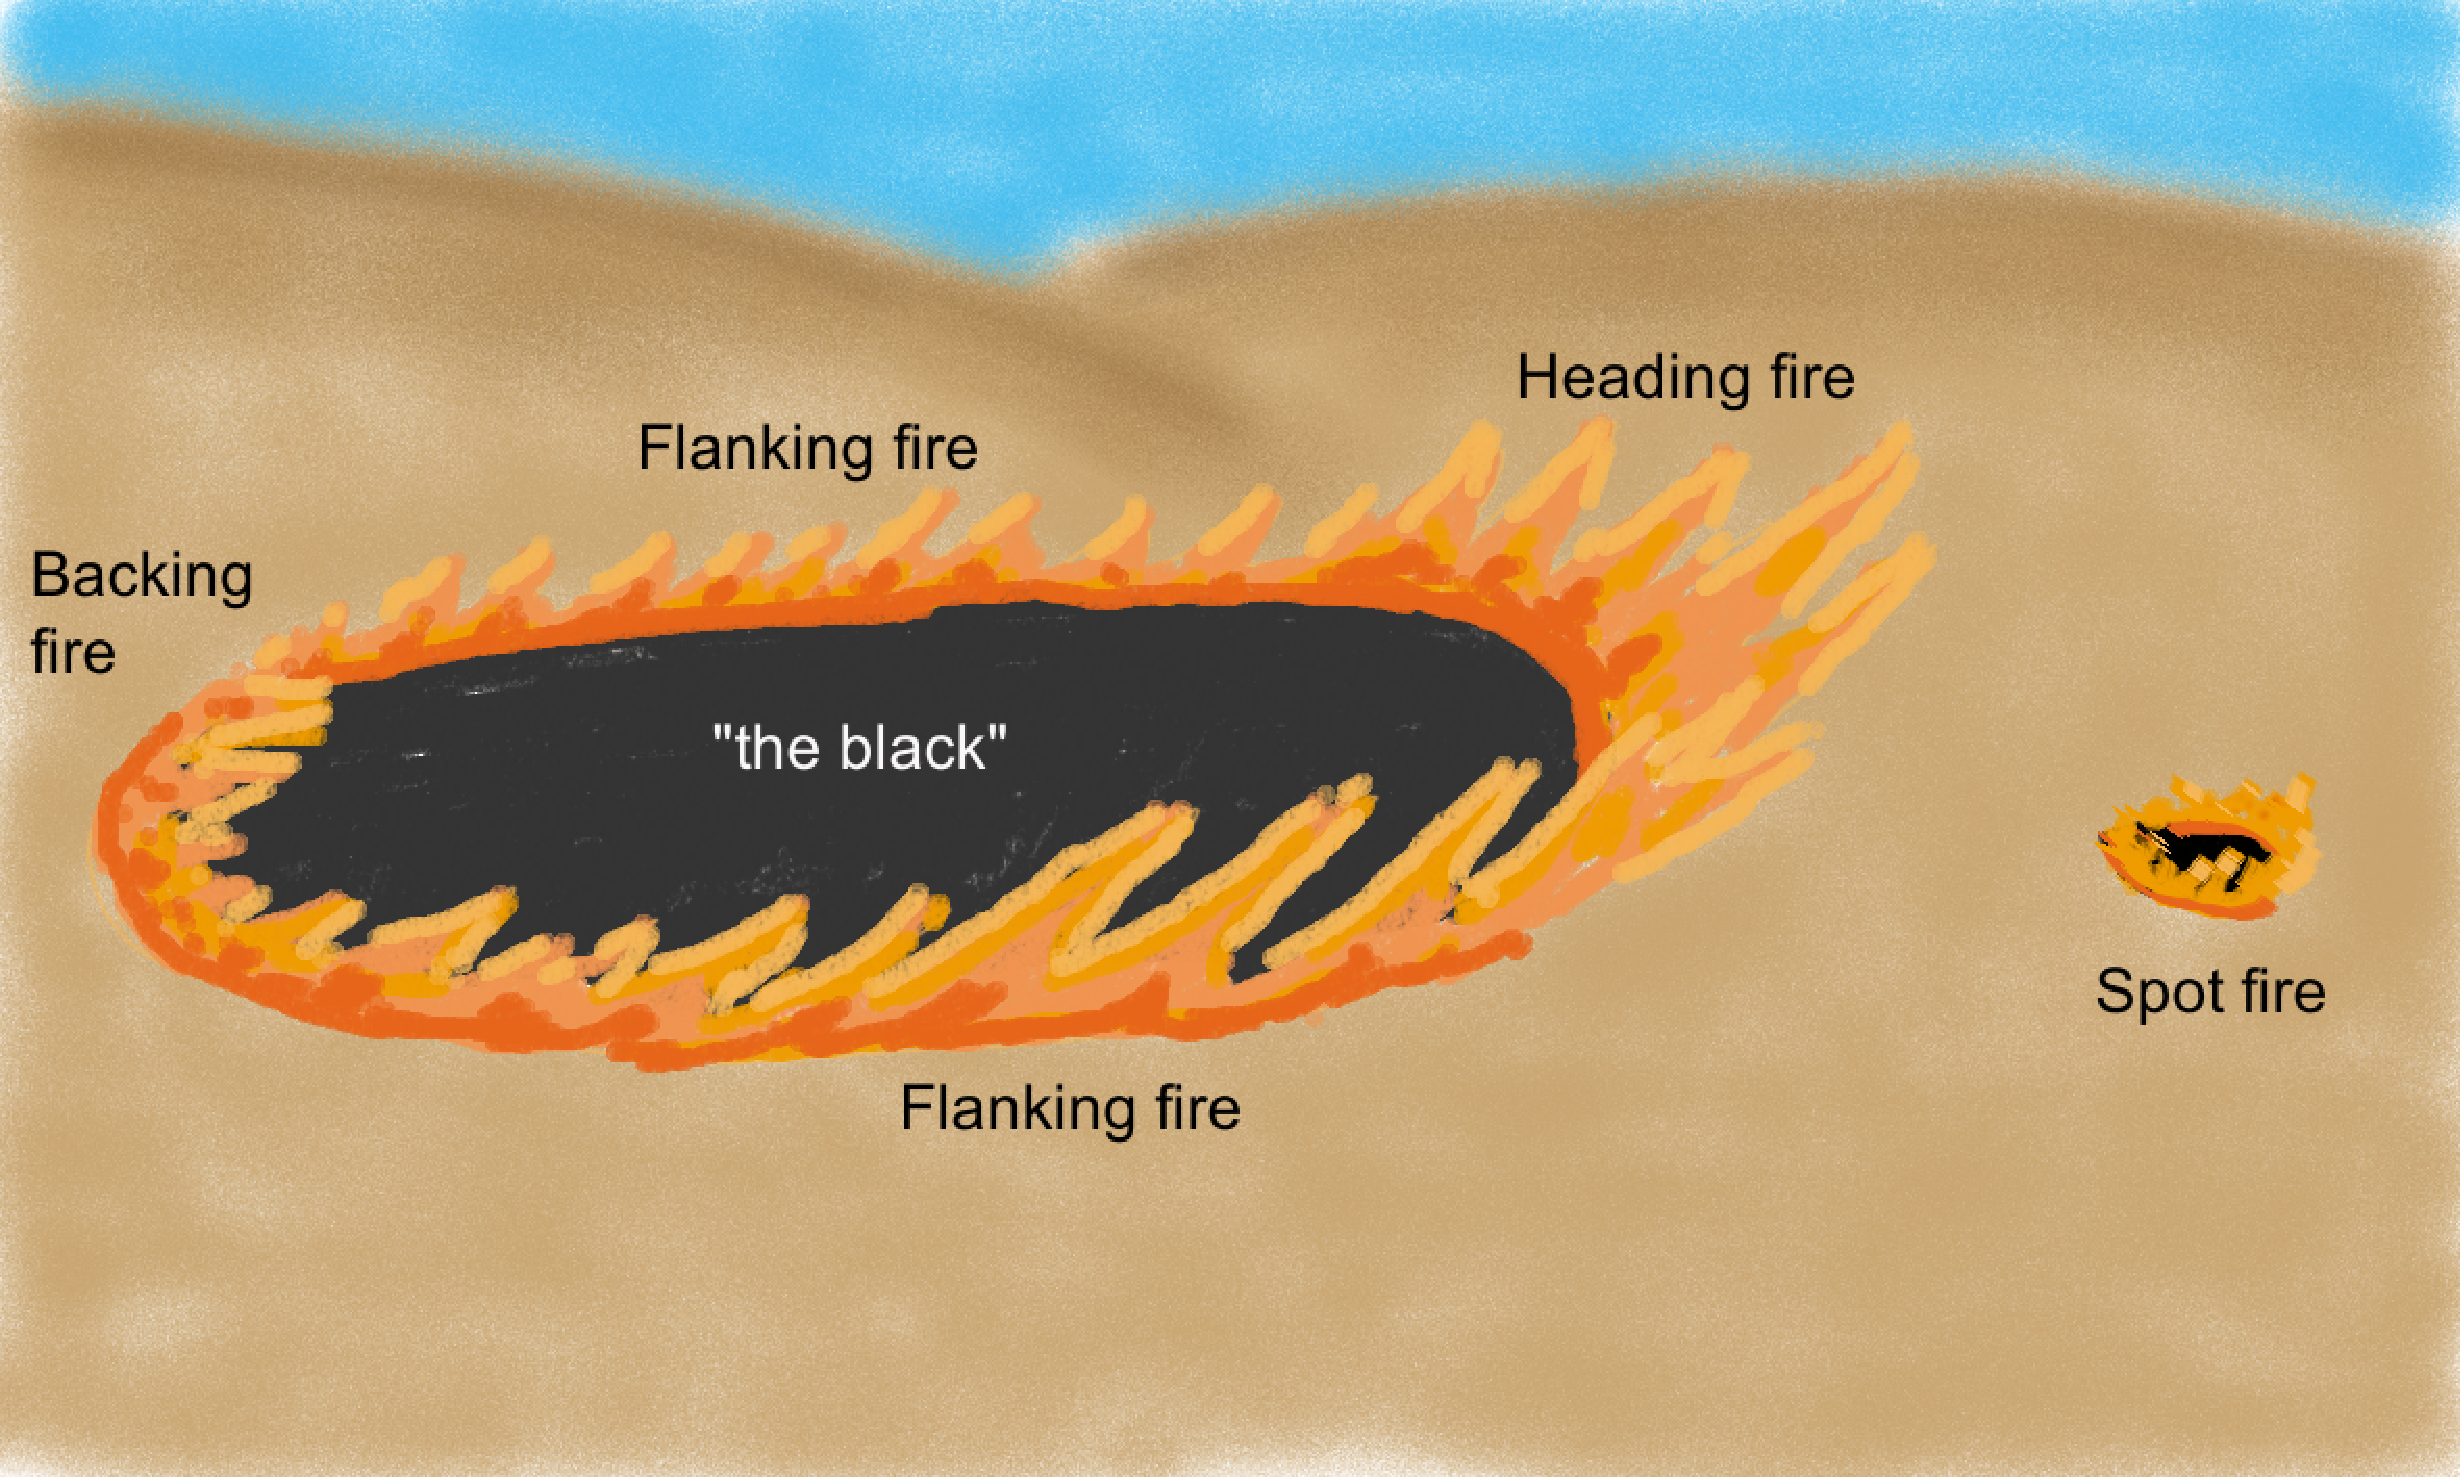
\includegraphics[width=1\textwidth, 
		trim={0cm 3cm 0cm 0cm}, clip=true]
		{science/FireAnatomy}
		%(Fig. \ref{fig:EllipseCartoon})
	\end{center}
\end{figure}

While fire \emph{spreads} outward as a flame front via propagation, \emph{fire growth} is driven by increases in burned area, including the spot fires that accelerate the increase in burned area beyond the spread of individual flame fronts.
On level terrain with a continuous, even fuelbed and constant wind, the shape of a fire's burned area depends primarily on wind speed.
The higher the wind speed, the longer and more narrow the burn perimeter.

A brief description of the anatomy of a wildland fire:

\begin{marginfigure}
	\begin{center}
		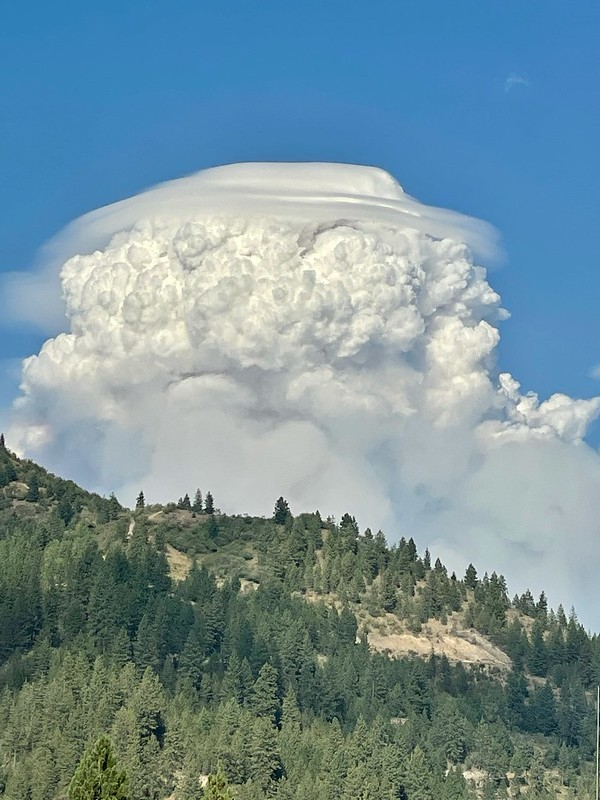
\includegraphics[width=1\textwidth, 
		                trim={0 0cm 0 0},clip=true]
		        {science/VeryLargePlume}
	% 	\PhotoCredit{ }
		\caption{Such a large smoke plume has developed over this wildfire that it has altered cloud formation at its top, several thousand feet above the fire.} 
		\label{fig:BigPlume} %(Fig.~\ref{fig:BigPlume})
	\end{center}
\end{marginfigure} 

\begin{itemize}
	\item \textbf{Head(ing) fires} move with the wind. 
Wind drives convective heat transfer by pushing warm air ahead of the fire,  which accelerates pre-heating, propagation, and fire spread.
\item \textbf{Backing fires} crawl into the wind. 
Blowing heat back over previously burned areas instead of into unburned fuel reduces preheating.
\item \textbf{Flanking fires} are the sides of the fire that burn parallel to the wind.
The lower intensity of flanking fires can be important tactically for wildland firefighters, as it is easier to fight these flames directly and work toward the head fire, reducing the total area burned.\footnote[][1cm]{Because a wind shift could easily turn a flanking fire into a head fire, it is important that personnel working on a flanking fire do so from the burned area within the perimeter, which serves as a safety zone.} 
\item \textbf{Spot fires} start via \emph{firebrands}\textemdash burning embers carried ahead of a flame front by wind or convection.
\item The \textbf{smoke plume} consists of the ``gases, smoke, and debris that rise slowly from a fire while being carried along the ground because the buoyant forces are exceeded by those of the ambient surface wind \citep{nwcg2019}.'' 
Plumes that develop strong updraft are called \emph{convective columns}, highlighting their effect on fire behavior (Fig.~\ref{fig:BigPlume}). 
Many fire-atmosphere interactions that relate to convective lift aren't directly visible. 
Plume structure provides insight into atmospheric conditions and plume properties such as color and roiling indicate fire behavior. 
\end{itemize} 

\subsection{Fire-atmosphere interactions}

Fires interact with the atmosphere. 
Crucially, these interactions are often simultaneously the least visible factors affecting fire behavior and the most important factors affecting the safety and effectiveness of prescribed burns. 
Thus it is important for all prescribed fire professionals to know how to read the signs that indicate how a fire is interacting with the invisible atmosphere. 

\begin{figure*}
	\caption{An illustration of general indicators of \emph{atmospheric stability}\textemdash the resistance of the atmosphere to mixing via vertical movement of air. 
		A stable atmosphere  resists mixing, which limits convective lift of smoke and generally subdues fire behavior. 
		An unstable atmosphere is receptive to rapid convection and smoke lift, which increases ventilation of the combustion reaction zone and increases fire intensity. 
		\label{fig:AtmopshericStability}  }
	\begin{center}
		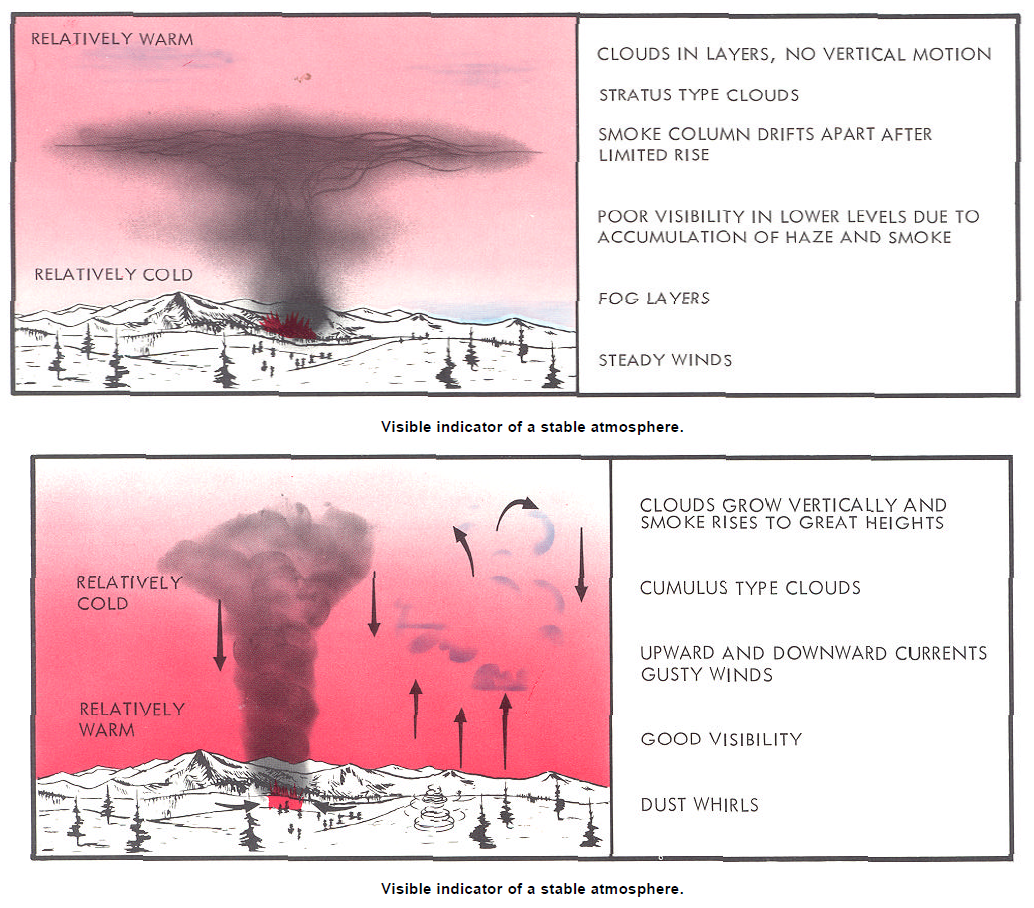
\includegraphics[width=1\textwidth, 
		trim={0cm 0cm 0cm 0cm}, clip=true]
		{science/AtmosphericStability}
		%(Fig. \ref{fig:AtmopshericStability})
			\PhotoCredit{\citet{schroeder1970}}
	\end{center}
\end{figure*}

	\index{Atmosphere!Atmospheric stability} 
\emph{Atmospheric stability} refers to how resistant the atmosphere is to vertical air movement, one of the controls on fire behavior \citep[][Fig. \ref{fig:AtmopshericStability})]{schroeder1970}. 
Hot combustion gasses and heated air are buoyant, and naturally seek to rise until the air expands and cools. 
In an unstable atmosphere, warm air rises easily, which increases convective airflow away from the combustion zone.
One cannot directly observe instability, but meteorologists can measure and predict associated variables. 
US fire weather forecasts include the \emph{Haines Index}, an index of the potential for rapid fire growth derived from correlations between observed fire behaviour and atmospheric stability \citep{haines1988}.
	\index{Haines Index}   
	
An \emph{inversion} is a departure from the typical pattern in which air gets colder with distance from the Earth's surface. 
\emph{Surface inversions} are deep layers of cool air near the surface, also known as \emph{night inversions} because such cooling often occurs at night \citep{schroeder1970}. 
Inversions form low, stable barriers of air that prevent mixing, convection, and smoke dispersal. 
Although inversions are prominent in mountainous regions, night inversions often form over broad areas without topography. 

The effect of an inversion on fire behavior is sometimes most noticeable as the inversion lifts.
By suppressing convection, inversions have the obvious effect of reducing the intensity of wildland fire burning under it, perhaps a prescribed fire lit during the morning. 
But as solar heating in the morning warms the surface, warm air begins to circulate in the near-surface atmosphere and starts to mix with higher layers. 
This convection and mixing weakens the inversion until it lifts entirely, allowing convective currents to reach to the top of the \emph{troposphere}, the lowest layer of the atmosphere that interacts with the Earth's surface. 
The consequence for fire behavior is greater intensity as convection develops.
 
\section{The fire regime} 

The fire regime of an area is the product of climate, vegetation, and the pattern of ignitions averaged over a given period of time (Fig.~\ref{fig:RegimeTriangle}). 
Many of the specific parameters of fire regimes\textemdash fire frequency, spatial extent, seasonality, intensity, and fire type\textemdash can also describe individual fire events. 

\begin{marginfigure}
	\begin{center}
		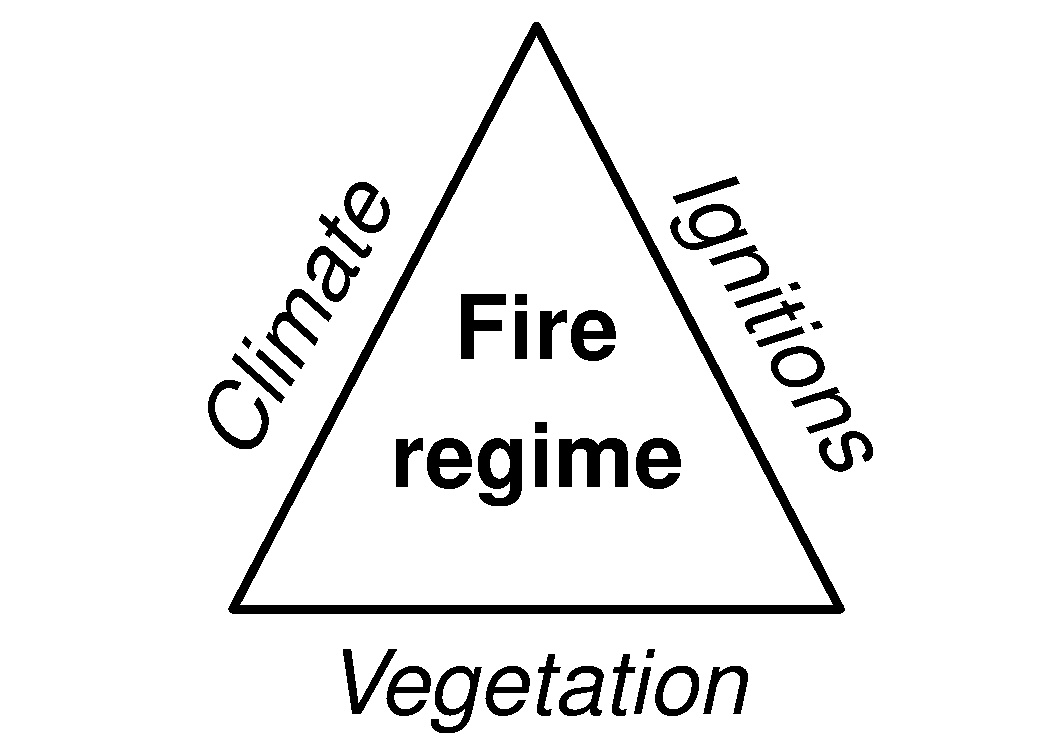
\includegraphics[width=2.2in, 
		trim={3cm 0cm 3cm 0},clip=true]
		{science/FireRegimeTriangle-1}
		\caption{The three sides of the Fire Regime Triangle.
			See Fig.~\ref{fig:ParametersFactors} for specific components with each side of the triangle.  }
		\index{Fire triangles!Fire regime|textit}
		\label{fig:RegimeTriangle} 	% (Fig.~\ref{fig:RegimeTriangle})
	\end{center}
\end{marginfigure} 

While the term \emph{fire regime} typically refers to a ``core group of parameters describing which fires occur when and where according to frequency, size, seasonality, intensity, and type'' \citep[][p. 61]{krebs2010}, many parameters are a product of two or more sides of the Fire Regime Triangle and are controlled at multiple temporal scales.

The importance of the fire regime concept to wildland fire science and management can hardly be overstated. 
The fire regime concept underpins the objectives of fire management policy as well as the strategy and tactics of prescribed fire operations (Fig.~\ref{fig:WalletCard}). 
Thus, to be useful, wildland fire scientists must target data collection to measure components of the wildland fire environment that relate to the targeted components of the fire regime.
Let us focus on the \emph{core parameters} of fire regime\textemdash the physical parameters of a specific fire, or the typical fire in an area. 

\begin{figure*} 
	%	\begin{center}
	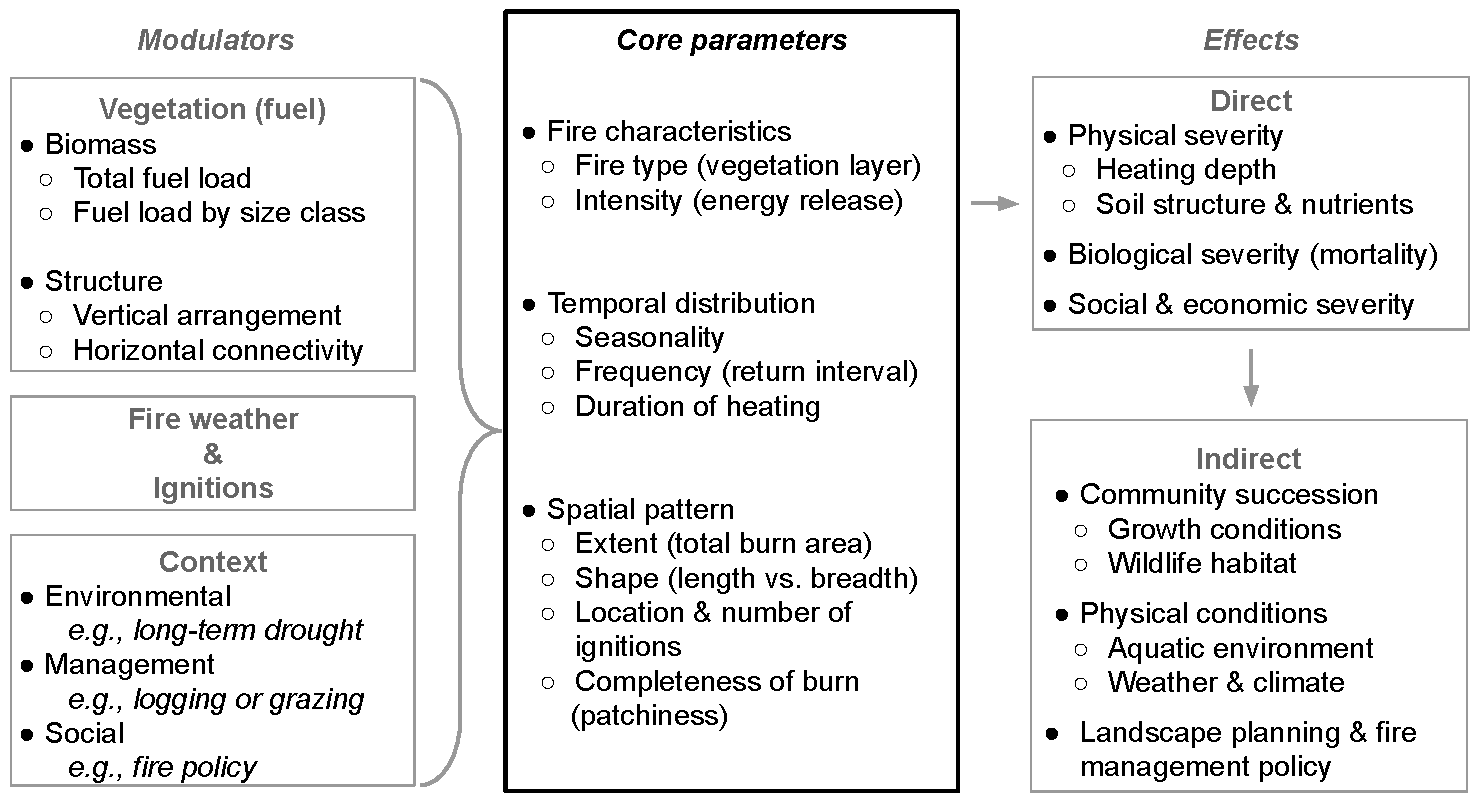
\includegraphics[width=0.85\paperwidth]
	{science/FireRegimeParts}
	\caption{
		The fire regime concept can be divided into core parameters\textemdash those that describe the physical characteristics of either one fire event, or the typical fire event\textemdash as well as biological, meteorological, and social factors that modulate fire events, and direct and indirect effects of fire. 
		Figure from \citet{mcgranahan2020}, inspired by \citet{krebs2010}. 
		\label{fig:ParametersFactors} }
	%(Fig.~\ref{fig:ParametersFactors})
	%	\end{center}
\end{figure*}

Two physical characteristics are important to fire regime: \emph{fire type} and \emph{fire intensity}, which describe the distribution of energy released to the environment, and where it might expose soil, plant organs, and organisms to heat.
Recall that fire type refers to the vegetation layer that burns (Fig.~\ref{fig:FireTypes}), and intensity refers to the energy released by the combustion of wildland fuel. 

There are three components to the timing of fire:

\begin{itemize}
	\item \textbf{Seasonality} describes when in the year a specific fire occurs, or when the typical fire is likely to occur. 
	It is broadly categorized as occurring in dormant or active seasons.
	Seasonality affects burn severity through direct and indirect interactions with \emph{phenology}\textemdash the timing of organisms' life histories relative to the climate.
	Generally, physiologically active organisms are more sensitive to fire damage. 
	\item \textbf{Fire frequency} typically means the number of fire events per period of time, while a similar term, \emph{fire return interval}, expresses time between fire events. 
	Both are measures of the amount of time between fire events, which affects both how long fuels have to accumulate and vegetation succession since the last disturbance. 
	\item \textbf{Duration of heating} refers to how long soil or organisms are exposed to elevated temperatures from combustion. 
	Many organisms have traits or behaviors that help them survive short periods of exposure to even high heat, but surviving long exposures to even moderate heat often requires specialized adaptations.
	Sometimes even just the difference between a fast-moving head fire or a slower backing fire creates variability in heat exposure in grassland. 
	Smoldering chunks of coarse fuels can hold heat against the soil. 
\end{itemize}

It is also important to consider the spatial pattern of fire. 
A simple measure is \emph{extent}, or the total area burned. 
\emph{Completeness of burn} refers to how much area within a fire perimeter actually burned. 
A fire with low burn completeness will have unburned areas where fire did not spread. 
Such areas might have been protected by fuel gaps created by streams or wetlands, rocky features, areas of intense herbivory, roads or trails, or defensive firebreaks. 
The resulting landscape is a patchwork of burned and unburned areas; thus \emph{patchiness} also describes the degree to which a fire did not burn completely.

\section{Accounting for environmental variability} 

One of the most basic principles of the scientific method is to focus on the variable of interest, and hold everything else constant. 
This is fairly easy in controlled experimental environments. 
For example, if a researcher wants to determine whether road dust effects photosynthesis in crop plants, they would find seeds from the same source, plant them at the same time in the same type of soil, give them the same water and fertilizer and the same amount of light in a greenhouse, and measure photosynthesis after applying dust to a randomly-selected group of plants (Fig.~\ref{fig:dust}). 
If there are differences in photosynthesis between the two groups, it is reasonable to assume that the differences are due to the dust, because everything else was held constant. 

\begin{marginfigure}
	\begin{center}
		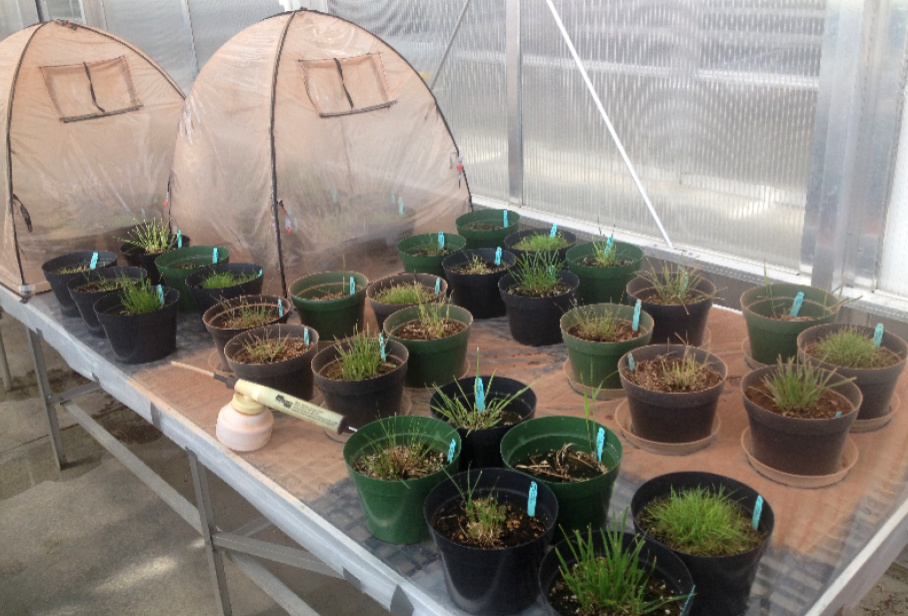
\includegraphics[width=2.2in, 
		trim={0cm 0cm 0cm 0cm}, clip=true]
		{science/GreenhouseDust}
		\caption{Controlled application of dust on plant leaves in a greenhouse. 
			\label{fig:dust} } 
		% \index{Fire triangles!Fire behaviour|textit}
		% (Fig.~\ref{fig:dust})
	\end{center}
\end{marginfigure}

But working out in the natural environment at the scales that land is managed is different. 
The environment is inherently variable\textemdash only the most highly-managed field or pasture has exactly the same time of plants in the same type of soil on the same slope and with the same amount of moisture. 
Wildlands and other areas managed for wildlife, native plants, and general biodiversity conservation are notoriously variable in terms of topography, soil, hydrology, and plant communities.
